\chapter{Capture des exigences fonctionnels}

\section{Diagramme des cas d'utilisation}
\begin{center}
	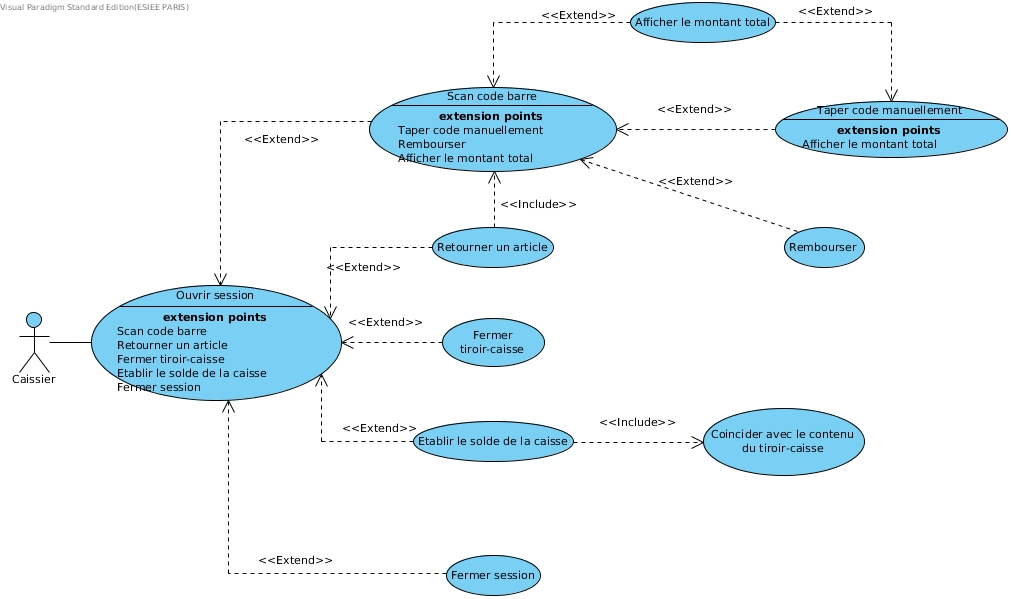
\includegraphics[width=14cm]{DiagrammeUseCaseCaisser.jpg}
\end{center}

\begin{center}
	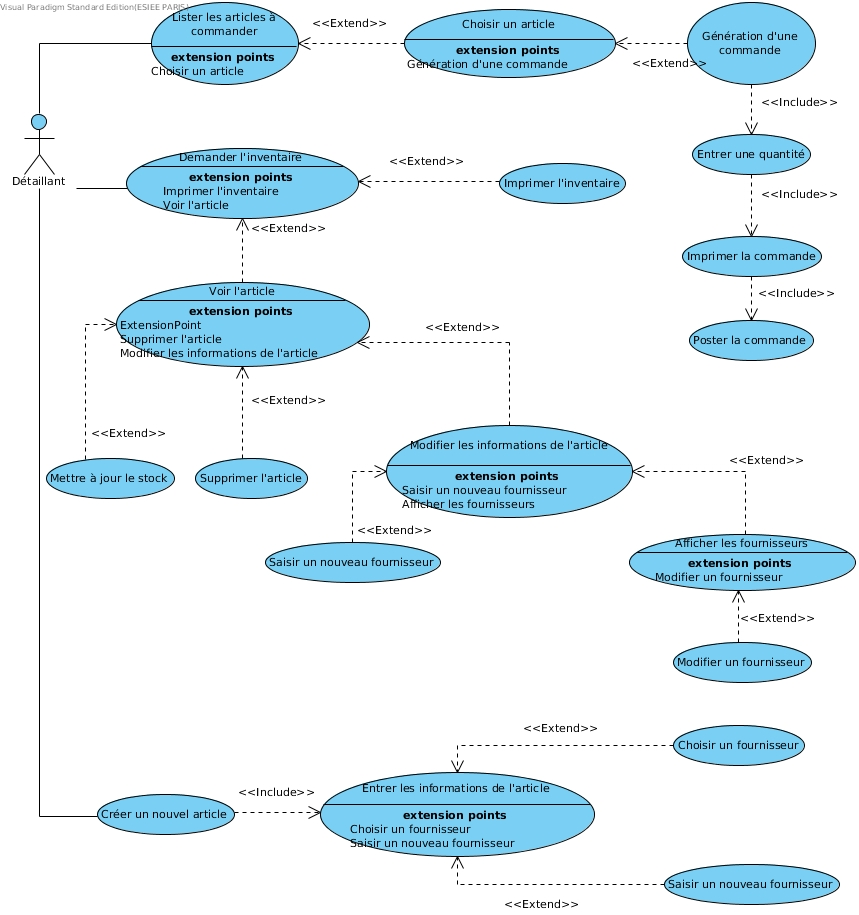
\includegraphics[width=14cm]{DiagrammeUseCaseDetaillant.jpg}
\end{center}

\section{Description des cas importants}

\subsection{Cas d'utilisation : Génération d'une commande}
\begin{itemize}
	\item Objectif : Commander des articles dont la quantité est passée sous un seuil définit
	\item Acteurs concernés : Le détaillant
	\item Pré conditions : La quantité de l'article est passée sous un seuil et le détaillant à choisi l'article en question dans la liste des articles dont le niveau en stock est inférieur au seuil définit.
	\item Scénario nominal :
		\begin{enumerate}
			\item Le détaillant affiche la liste des articles dont le niveau de stock est inférieur au seuil définit
			\item Le détaillant sélectionne l'article qui veut commander
			\item Le détaillant valide la commande
		\end{enumerate}
\end{itemize}

\subsection{Cas d'utilisation : Mettre à jour le stock}
\begin{itemize}
	\item Objectif : Mettre à jour le stock d'un article
	\item Acteurs concernés : Le détaillant
	\item Pré conditions : Le détaillant a sélectionné l'article concerné dans l'inventaire et a sélectionné l'option d'édition de l'article
	\item Scénario nominal :
	\begin{enumerate}
		\item Le détaillant demande l'inventaire des stocks
		\item Le détaillant sélectionne l'article dont le niveau de stock doit être mis à jour
		\item Le détaillant sélectionne l'option d'édition
		\item Le détaillant modifie le niveau de stock
	\end{enumerate}
\end{itemize}


\subsection{Cas d'utilisation : Saisir un nouveau fournisseur}
\begin{itemize}
	\item Objectif : Ajouter un fournisseur à un article
	\item Acteurs concernés : Le détaillant
	\item Pré conditions : Le détaillant a sélectionné l'article concerné dans l'inventaire et a sélectionné l'option d'édition de l'article
	\item Scénario nominal :
	\begin{enumerate}
		\item Le détaillant demande l'inventaire des stocks
		\item Le détaillant sélectionne l'article
		\item Le détaillant sélectionne l'option d'édition
		\item Le détaillant rajoute un fournisseur avec ses informations
	\end{enumerate}
\end{itemize}

\subsection{Cas d'utilisation : Scan d'un code barre}
\begin{itemize}
	\item Objectif : Scanner un article
	\item Acteurs concernés : Le caissier
	\item Pré conditions : Le caissier a démarré une session sur la caisse et un client s'est présenté devant la caisse avec un article.
	\item Scénario nominal :
	\begin{enumerate}
		\item Le caissier ouvre une session sur la caisse
		\item Un client approche avec un article
		\item Le caissier scan le code barre de l'article
	\end{enumerate}
	
	\item Scénario alternatif :
	\begin{enumerate}
		\item Le caissier ouvre une session sur la caisse
		\item Un client approche avec un article
		\item Le code barre est illisible et le caissier entre la référence de l'article puis appuie sur <Enter>
	\end{enumerate}
\end{itemize}

\subsection{Cas d'utilisation : Remboursement d'un article}
\begin{itemize}
	\item Objectif : Remboursement d'un article
	\item Acteurs concernés : Le caissier
	\item Pré conditions : Le caissier a démarré une session sur la caisse et un client s'est présenté devant la caisse avec un article à retourner. L'article doit être vendable.
	\item Scénario nominal :
	\begin{enumerate}
		\item Le caissier ouvre une session sur la caisse
		\item Un client approche avec un article à retourner
		\item L'article en question est vendable
		\item Le caissier scan le code barre de l'article
		\item Le tiroir de la caisse s'ouvre
		\item Le caissier rembourse le client
	\end{enumerate}
	
	\item Scénario alternatif 1
	\begin{enumerate}
		\item Le caissier ouvre une session sur la caisse
		\item Un client approche avec un article à retourner
		\item L'article n'est pas vendable et le client ne se fait pas rembourser
	\end{enumerate}
	
	\item Scénaio alternatif 2
	\begin{enumerate}
		\item Le caissier ouvre une session sur la caisse
		\item Un client approche avec un article à retourner
		\item L'article en question est vendable
		\item L'article est vendabe et le code barre est illisible.
		\item Le caissier entre alors la référence de l'article puis appuie sur <Enter>. 
		\item Le tiroir de la caisse s'ouvre
		\item Le caissier rembourse le client
	\end{enumerate}
\end{itemize}

\subsection{Cas d'utilisation : Solde de la caisse}
\begin{itemize}
	\item Objectif : Effectuer le solde de la caisse
	\item Acteurs concernés : Le caissier
	\item Pré conditions : Le caissier a démarré une session sur la caisse et appuie deux fois sur <Total>
	\item Scénario nominal :
	\begin{enumerate}
		\item Le caissier ouvre une session sur la caisse
		\item Le caissier appuie deux fois sur la touche <Total>
		\item Le tiroir de la caisse s'ouvre et la caisse lance l'impression de la liste des tickets de caisse.
		\item Le caissier fait coïncider le contenu du tiroir de caisse avec le montant total de l'ensemble des opréations réalisées.
	\end{enumerate}
\end{itemize}




\section{Prototypes des interfaces}

\subsection{Vue de l'accueil backend}
\begin{center}
	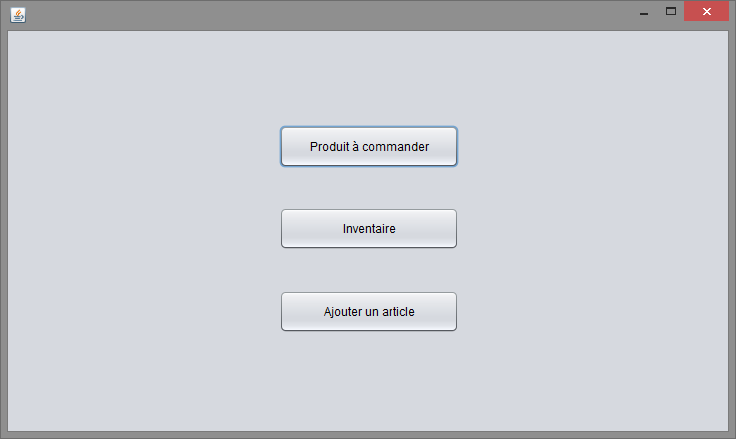
\includegraphics[width=14cm]{HomeView.png}
\end{center}

\subsection{Vue de l'inventaire}
\begin{center}
	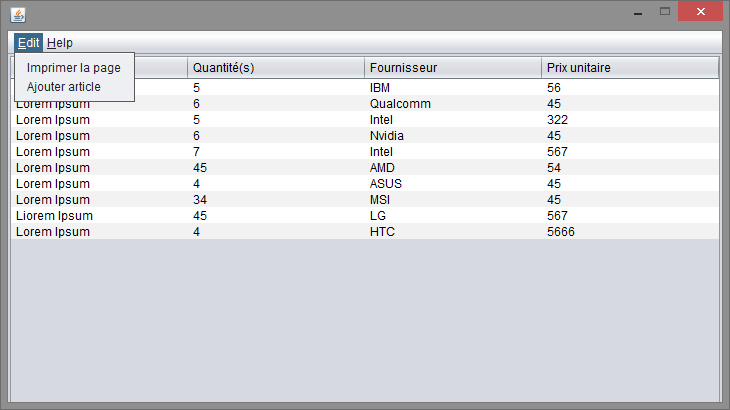
\includegraphics[width=14cm]{InventaireView.png}
\end{center}

\subsection{Vue d'un article}
\begin{center}
	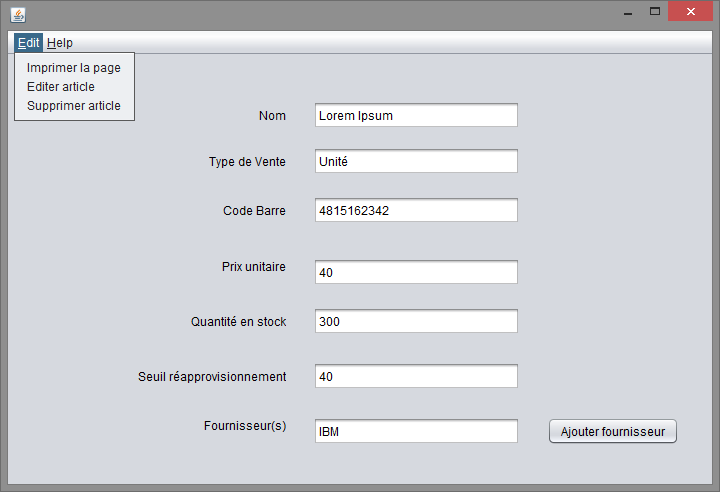
\includegraphics[width=14cm]{ArticleView.png}
\end{center}

\subsection{Vue d'ajout et d'édition d'un article}
\begin{center}
	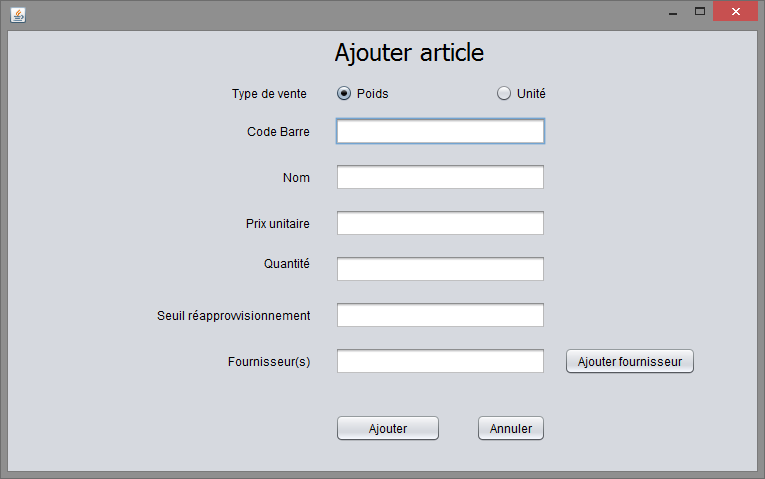
\includegraphics[width=14cm]{FormArticle.png}
\end{center}

\subsection{Vue d'ajout et d'édition d'un fournisseur}
\begin{center}
	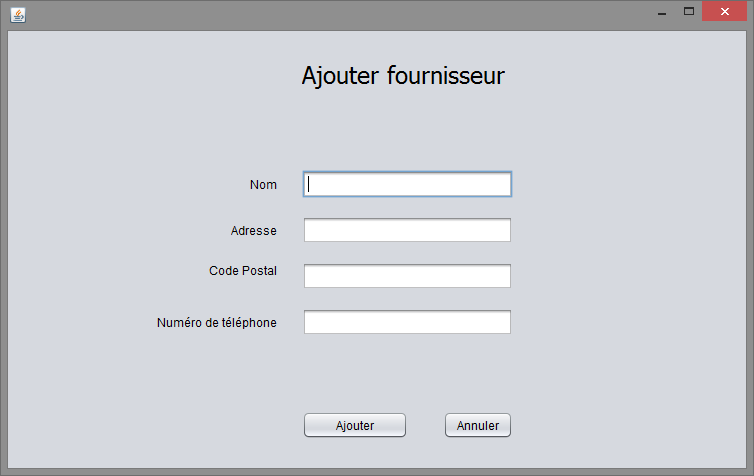
\includegraphics[width=14cm]{FormFournisseur.png}
\end{center}

\subsection{Vue d'une commande}
\begin{center}
	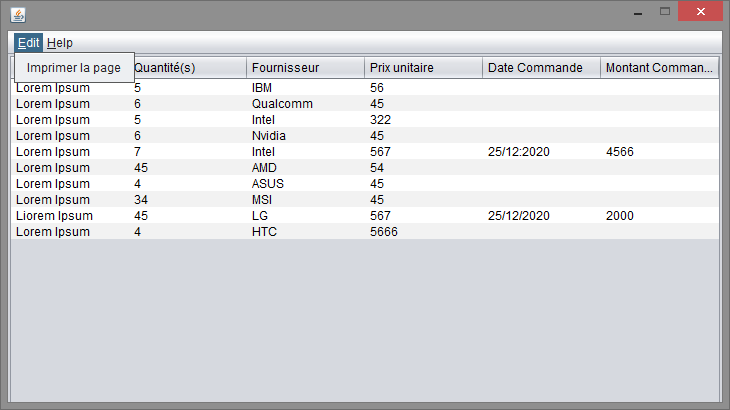
\includegraphics[width=14cm]{CommanderView.png}
\end{center}

\subsection{Vue pour passer une commande}
\begin{center}
	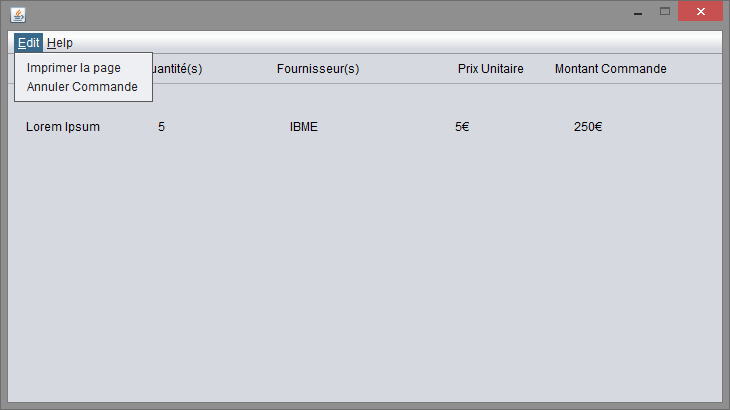
\includegraphics[width=14cm]{CommandeView.png}
\end{center}

\subsection{Vue de la caisse}
\begin{center}
	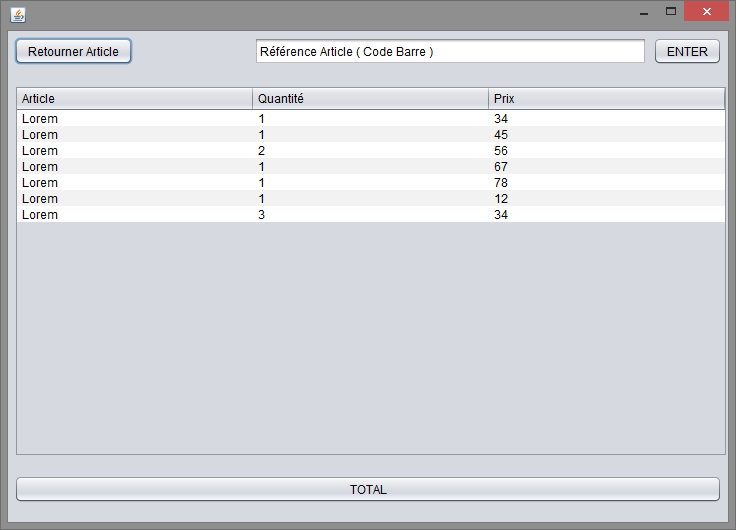
\includegraphics[width=14cm]{CaisseView.png}
\end{center}


%---------------------------------------------------------------
\chapter{Etude du modèle statique}

\section{Diagramme de classe}
\begin{center}
	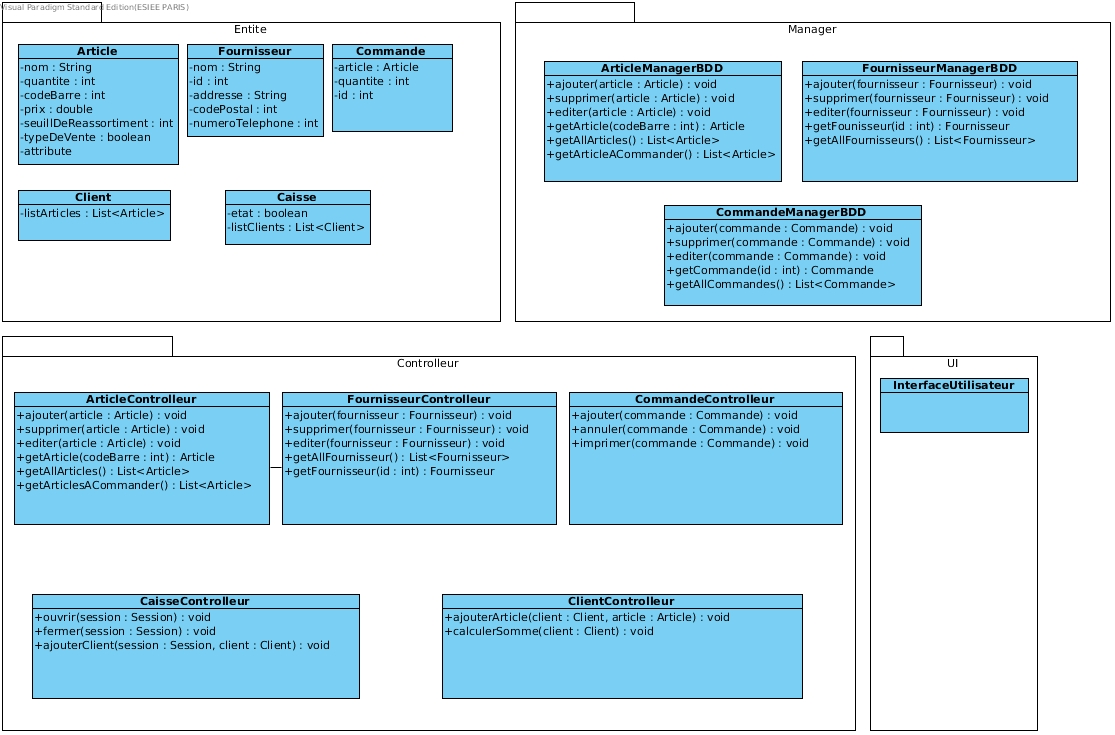
\includegraphics[width=14cm]{DiagrammeDeClasseEbauche.jpg}
\end{center}

\section{Dictionnaire de données}

\subsection{Articles}

\subsubsection{Article}
La classe article décrit les caractéristiques d'un article : son identifiant, nom, prix et quantité en stock.
Cette classe sera instanciée autant de fois qu'il y aura d'article différent.

\subsubsection{ArticleController}
La classe ArticleController effectue toutes les actions sur les objets articles : retourner une liste d'objets, traiter des objets etc ...
 Elle ne sera instanciée qu'une seule fois.
 
\subsubsection{ArticleMananger}
ArticleManager fait le lien entre la base de donnée et les entitées Articles. Elle sera également instanciée qu'une seule fois. Ses fonctions essentiels sont la sauvegarde, l'ajout et l'édition d'un article dans la base de donnée.

\subsection{Fournisseur}

\subsubsection{Fournisseur}
La classe Fournisseur décrit les caractéristiques d'un article : son nom et son identifiant. La classe fournisseur sera instanciée autant de fois qu'il y aura de fournisseur différent.

\subsubsection{FournisseurController}
La classe FournisseurController effectue toutes les actions sur les objects : retourner une liste, suppression, édition etc ...
Elle ne sera instanciée qu'une seule fois.

\subsubsection{FournisseurMananger}
FournisseurManager fait le lien entre la base de donnée et les entitées Fournisseur. Elle sera également instanciée qu'une seule fois. Ses fonctions essentiels sont la sauvegarde, l'ajout et l'édition d'un fournisseur dans la base de donnée.

\subsection{Commande}
\subsubsection{Commande}
La classe Commande décrit les caractéristiques d'une Commande : sa référence, les articles commandés et leur quantité. La classe Commande sera instanciée autant de fois qu'il y aura de commande différentes.

\subsubsection{CommandeController}
La classe CommandeController effectue toutes les actions sur les commandes: retourner la liste des commandes, annulation ...
Elle ne sera instanciée qu'une seule fois.

\subsubsection{CommandeMananger}
CommandeManager fait le lien entre la base de donnée et les entitées Commande. Elle sera également instanciée qu'une seule fois. Ses fonctions essentiels sont la sauvegarde, l'ajout et l'édition d'une Commande dans la base de donnée.

\subsection{InterfaceUtilisateur}
L'interfaceUtilisateur sera le controller principal des vues. Il instanciera et affichera toutes les vues décritent dans la partie précédente.

\subsection{Caisse}
L'objet caisse représente la caisse. Il contiendra en attribut les différents états de la caisse. La caisse sera instancié qu'une seule fois.

\subsection{Client}
\subsubsection{Client}
L'object Client répresente un client passant en caisse. Cette classe se chargera de retenir tous les articles achetés par un client. Elle sera donc instanciée autant de fois que de client passeront à la caisse.

\subsubsection{ClientController}
Comme toujours, le ClientController effectuera les actions sur les objects Clients. Cette classe sera instanciée qu'une seule fois.

\subsection{Caisse}

\subsubsection{Caisse}
La classe objet Caisse représente une session de la caisse. Elle sera instanciée autant de fois qu'un caissier démarrra une nouvelle session. Elle contiendra tous les états de la caisse et la liste des clients qui se seront présenté devant la caisse.

\subsubsection{CaisseController}
La classe CaisseController effectue toutes les actions sur les caisses: ouverture du tiroir, impression des tickets de caisse etc ...
Elle ne sera instanciée qu'une seule fois.


%---------------------------------------------------------------
\chapter{Etude du modèle dynamique}

\section{Diagramme de séquence et diagramme de classe des principaux cas d'utilisation}

\subsection{Diagramme de séquence et de classe pour le cas d'utilisation : Modifier les informations d'un article}
\begin{center}
	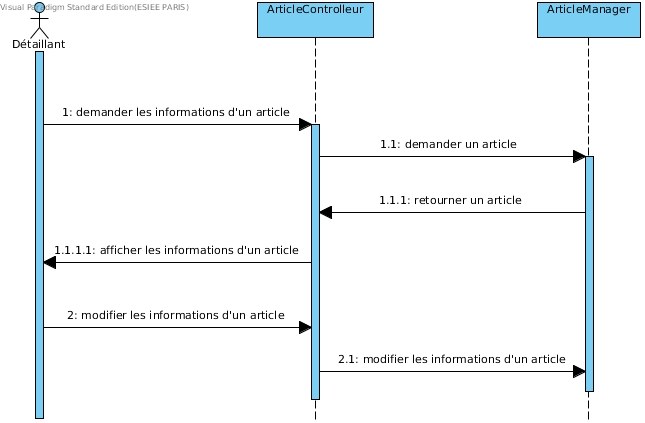
\includegraphics[width=14cm]{DiagrammeSequenceModifierInfoArticle.jpg}
\end{center}
\begin{center}
	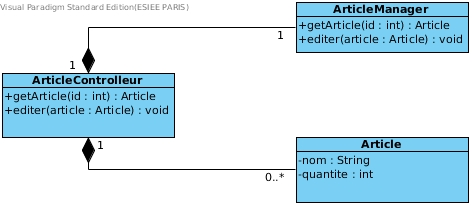
\includegraphics[width=14cm]{DiagrammeDeClasseModifierInfoArticle.jpg}
\end{center}

\subsection{Diagramme de séquence et de classe pour le cas d'utilisation : Lister les articles à commander}
\begin{center}
	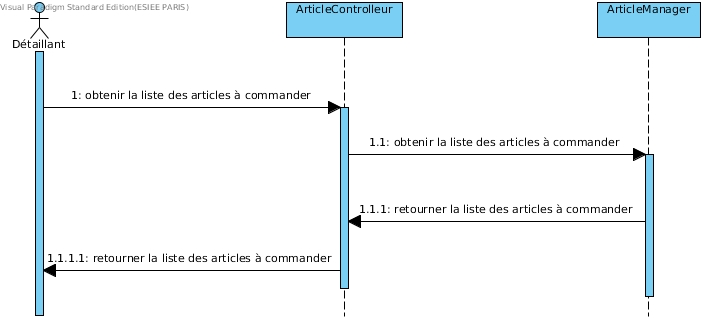
\includegraphics[width=14cm]{DiagrammeSequenceListerArticlesACommander.jpg}
\end{center}
\begin{center}
	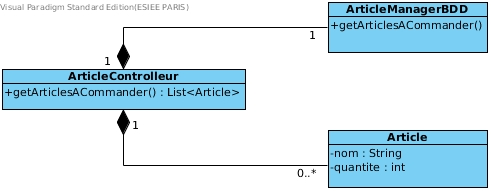
\includegraphics[width=14cm]{DiagrammeDeClasseListerArticlesACommander.jpg}
\end{center}


\section{Diagramme d'états de certaines classes pertinentes}

\subsection{Diagramme d'état d'un article}
\begin{center}
	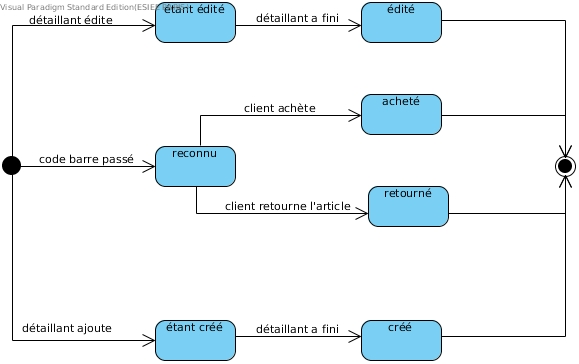
\includegraphics[width=14cm]{DiagrammeEtatArticle.jpg}
\end{center}

\subsection{Diagramme d'état de la caisse}
\begin{center}
	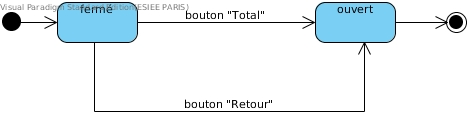
\includegraphics[width=14cm]{DiagrammeEtatCaisse.jpg}
\end{center}


\chapter{Synthèse}
\begin{center}
	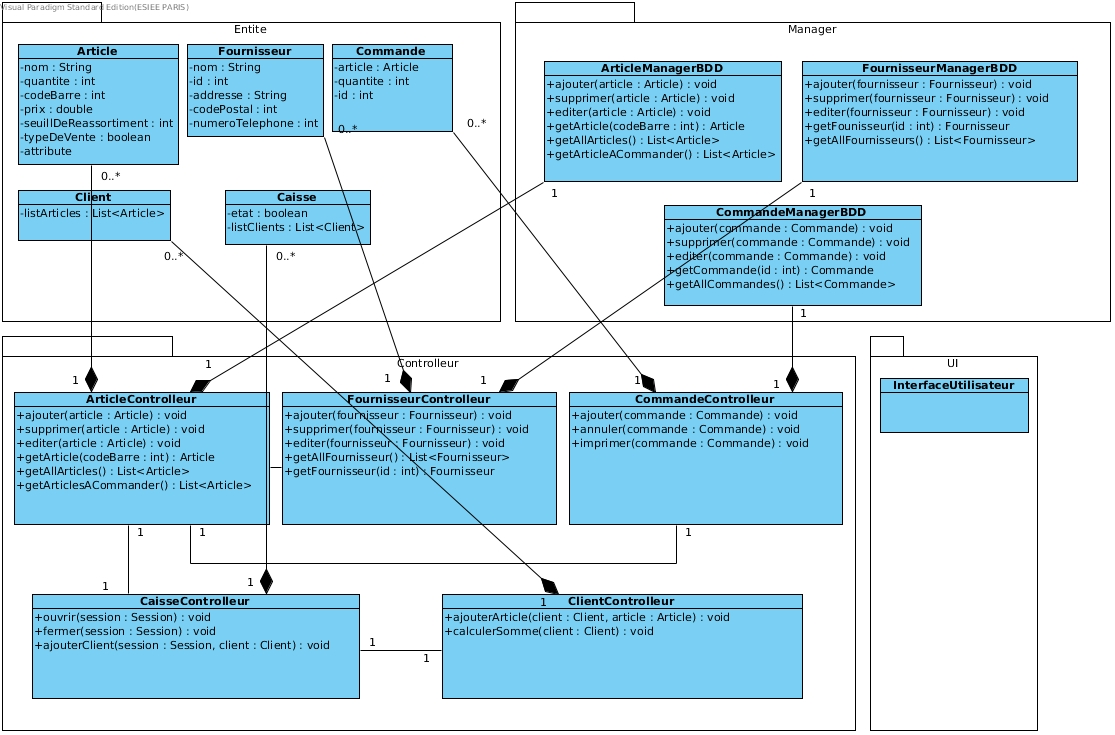
\includegraphics[width=15cm]{DiagrammeDeClasse.jpg}
\end{center}


	